\documentclass[11pt,oneside,dvipdfmx]{jbook}
\usepackage{it_thesis}

\usepackage{graphicx}
\usepackage{amsmath,bm} 
\usepackage{amssymb}
\usepackage{amsfonts}
\usepackage{array}
\usepackage{subfig}
\usepackage[utf8]{inputenc}
\usepackage{color}
\usepackage{xcolor}
\usepackage{colortbl}
\usepackage{url}
\usepackage{otf}
%\usepackage{remreset}
\usepackage{cite}
\usepackage{pdfpages}

\usepackage{here}
\usepackage[top=30truemm,bottom=20truemm,left=30truemm,right=20truemm]{geometry}
%\usepackage[font=large]{caption}
\usepackage{times}
\usepackage{layout}
\usepackage{booktabs}
\usepackage{multirow}
\usepackage{ulem}
\usepackage{algorithm}
\usepackage{algorithmicx}
\usepackage{algpseudocode}
\usepackage{enumitem}
\usepackage{wrapfig}

% 添削時は以下は使わないこと
%\usepackage[dvipdfmx]{hyperref}
%\usepackage{pxjahyper}
%\usepackage[dvipdfmx]{pdfcomment}

% 必要なpackageは以下に追加

\makeatletter\@removefromreset{footnote}{chapter}\makeatother

\newcommand{\doi}[1]{\url{https://doi.org/#1}}

\newcommand{\note}[1]{{\color{blue} {\it #1} }}

\DeclareMathAlphabet{\mathsf}{OT1}{\sfdefault}{m}{n}
\SetMathAlphabet{\mathsf}{bold}{OT1}{\sfdefault}{b}{n}

\newcommand{\tens}[1]{\ensuremath{\boldsymbol{\mathsf{#1}}}}
\newcommand{\vect}[1]{\ensuremath{\boldsymbol{#1}}}
\newcommand{\set}[1]{\ensuremath{\mathcal{#1}}}

% Math operators
\newcommand{\diff}[2]{\frac{d {#1}}{d {#2}}}
\newcommand{\pdiff}[2]{\frac{\partial {#1}}{\partial {#2}}}
\newcommand{\restrict}[2]{\left. {#1} \right|_{#2}}
\DeclareMathOperator{\tr}{tr}
\DeclareMathOperator{\dev}{dev}
\DeclareMathOperator{\diag}{diag}
\DeclareMathOperator{\sgn}{sgn}
\newcommand{\argmin}{\mathop{\rm arg~min}\limits}

% vectors
\newcommand{\vf}{\vect{f}}
\newcommand{\vp}{\vect{p}}
\newcommand{\vw}{\vect{w}}
\newcommand{\vz}{\vect{z}}


\newcommand{\vwk}{{\vw^{(k)}}}
\newcommand{\vzk}{{\vz^{(k)}}}
\newcommand{\vzkone}{{\vz^{(k+1)}}}
\newcommand{\vzzero}{{\vz^{(0)}}}
\newcommand{\vzstar}{{\vz^{*}}}

% tensors
\newcommand{\tZ}{\tens{Z}}

% sets
\newcommand{\sW}{\set{W}}


% Algorithm
\renewcommand{\algorithmicrequire}{\textbf{Input:}}  % Use Input in the format of Algorithm
\renewcommand{\algorithmicensure}{\textbf{Output:}} % Use Output in the format of Algorithm
\newcommand{\algorithmautorefname}{Algorithm}

\algnewcommand{\algorithmicand}{\textbf{ and }}
\algnewcommand{\algorithmicor}{\textbf{ or }}
\algnewcommand{\Or}{\algorithmicor}
\algnewcommand{\And}{\algorithmicand}
\algnewcommand{\algorithmictrue}{\textbf{true}}
\algnewcommand{\True}{\algorithmictrue}


\renewcommand{\bibname}{参考文献}


%卒業年度（全角）
\year{２０２５}

%学年
%  学部4年生 -> B4
%  修士2年生 -> M2
\grade{B4}

%研究題目
\title{
    髭密度を考慮した
    皮膚表面下散乱モデルの提案
}
%% 副題
\subtitle{
 %副題がない場合はこの行のみを削除．\subtitle 自体はコメントアウト・削除しない．
}

% 提出日を作成（全角）
\date{２０２４年１月２２日提出}

% 指導教員名
\teacher{
楽　詠\UTF{705D}
}

% 学籍番号，氏名（いずれも全角）
\author{１５８２２１３３ 山本 雷夏}
\西暦
\begin{document}

% タイトルページの出力
\maketitle

\large
\setcounter{page}{0}
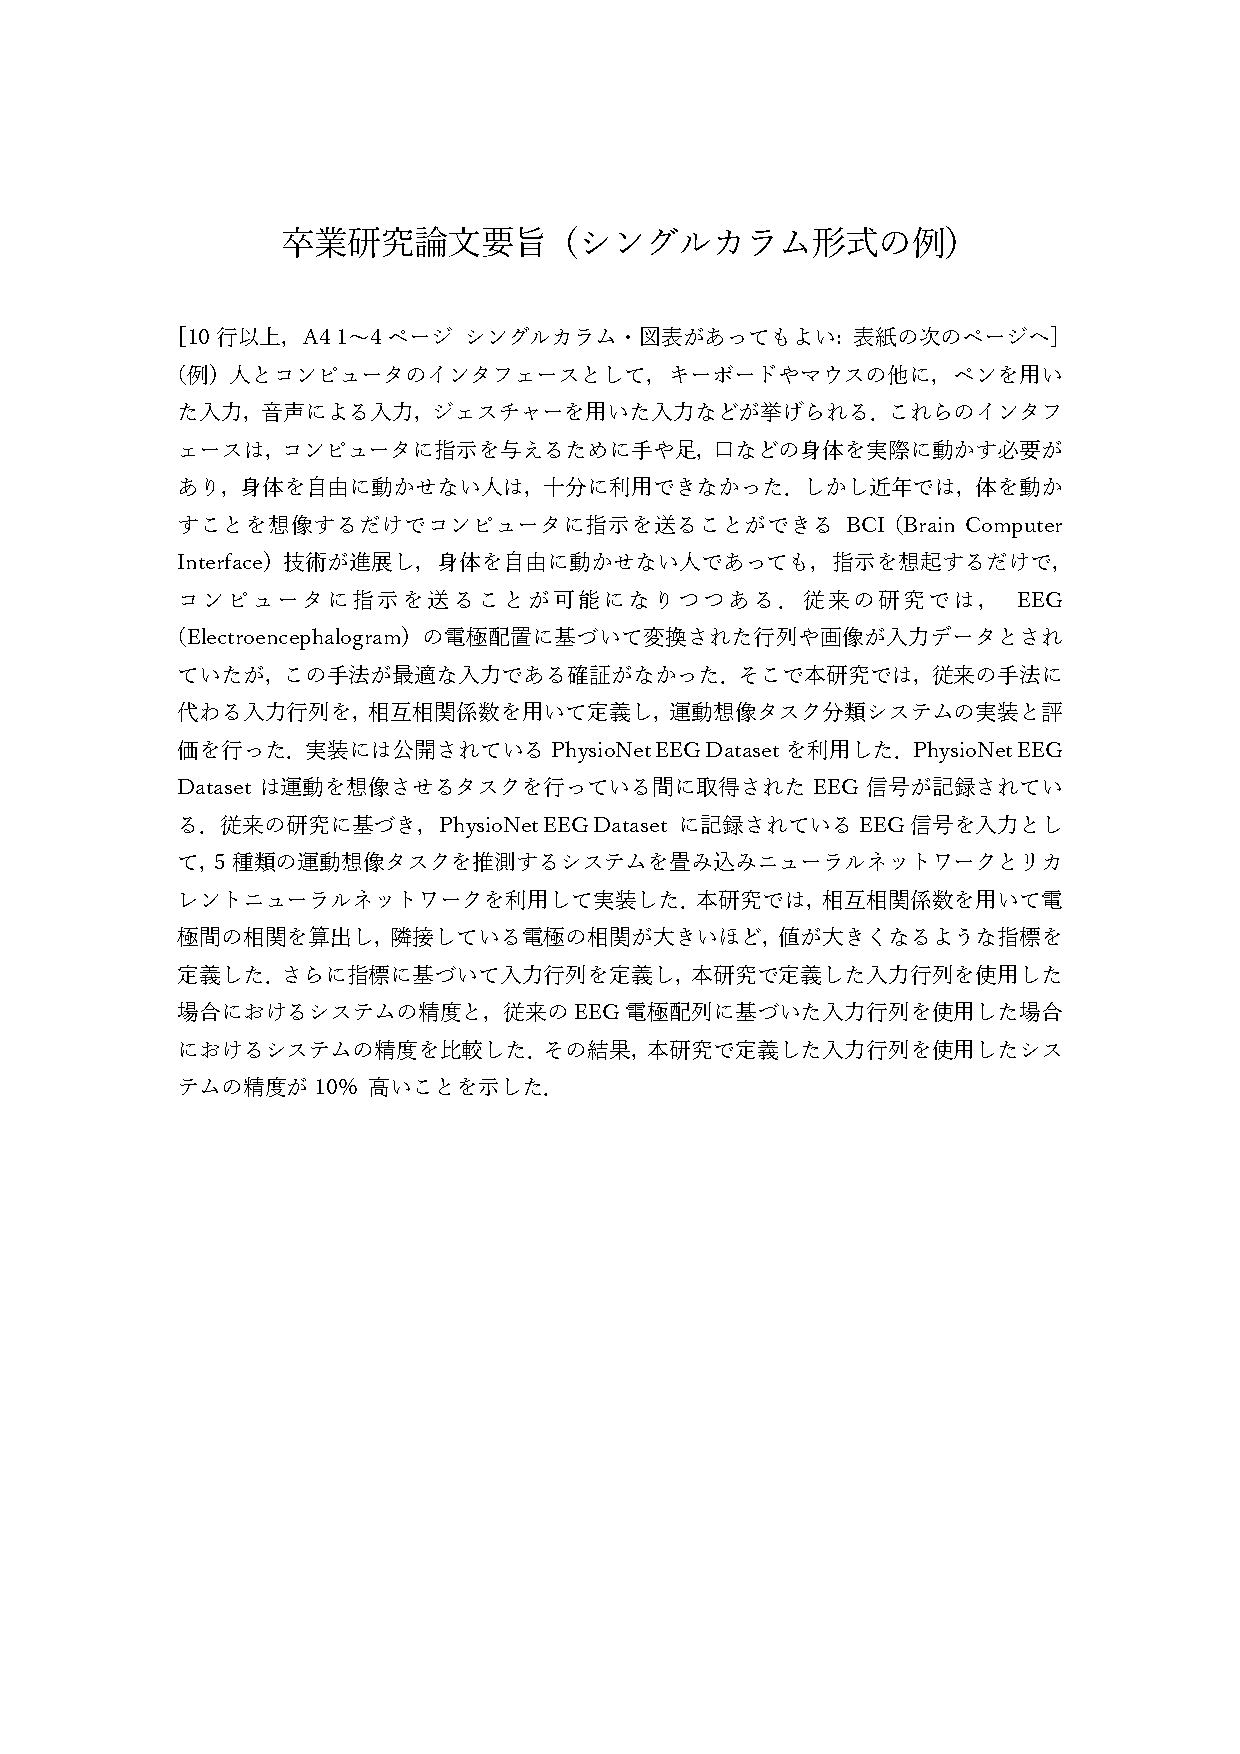
\includepdf[pages=-]{figs/youshi.pdf}

% 前置き部分（目次部分）の出力
\frontmatter
\pagestyle{plain}

%目次の出力
\tableofcontents

% 図目次を出力する場合，次の行を有効にする（コンパイルは2回すること） 
%\listoffigures

% 表目次を出力する場合，次の行を有効にする（コンパイルは2回すること）
%\listoftables

\clearpage

%本文の始まり
\mainmatter 

\chapter{はじめに}
\label{cha:introduction}

\section{研究背景}
近年，コンピュータグラフィックス技術の発展に伴い，
人物の顔を対象とした写実的な画像生成が
映画，ゲーム，VR/AR などの分野で広く用いられている。
これらの応用において，
人間の皮膚の質感をどれだけ現実に近づけられるかは，
映像全体のリアリティを左右する重要な要素である。

皮膚の見えに大きな影響を与える要因の一つとして，
皮膚内部で生じる表面下散乱が挙げられる。
表面下散乱は，
光が皮膚表面から内部に侵入し，
内部で複数回散乱した後，
異なる位置から出射する現象であり，
皮膚特有の柔らかさや透明感を生み出す。
この現象を表現するため，
従来から双方向表面下散乱反射率分布関数
(BSSRDF) を用いた研究が行われてきた。

一方で，人間の顔には皮膚だけでなく，
眉毛や髭といった毛髪構造が局所的に存在している。
特に髭は，
口周りや顎といった限られた領域に高密度で分布し，
皮膚表面付近で光を吸収・遮蔽する。
そのため，髭が存在する領域では，
皮膚のみの場合とは異なる
光のにじみや明度分布が観測される。

\section{研究課題}
従来の皮膚表面下散乱モデルの多くは，
皮膚を一様な媒質として近似しており，
髭のような局所的な構造物の影響は
明示的には考慮されていない。
その結果，
髭の生えている領域においても
皮膚のみの場合と同様の散乱特性が適用され，
見えが不自然になる場合がある。

髭の影響を厳密に扱うためには，
毛髪一本単位のジオメトリや，
異方的な散乱特性を考慮した
高度なモデルを導入する必要がある。
しかし，そのような手法は
計算コストが高く，
実用的なレンダリングへの適用が難しい。

したがって，
髭の存在による影響を
過度な計算コストを増加させることなく，
皮膚表面下散乱モデルに取り込む手法が求められている。

\section{本研究の目的と貢献}
本研究の目的は，
皮膚表面下散乱モデルに
髭の分布情報を導入することで，
髭の存在による見えの変化を
より現実的に表現することである。

具体的には，
髭の分布を髭密度として定義し，
この密度に基づいて
皮膚モデルと髭モデルを混合する
表面下散乱モデルを提案する。
本手法では，
髭をジオメトリとして直接扱うことなく，
密度マップとして集約することで，
計算効率と表現力の両立を図る。

本研究の主な貢献は以下の通りである。
\begin{itemize}
  \item 髭密度に基づいて皮膚表面下散乱特性を制御する混合モデルの提案
  \item 髭分布をテクスチャとして表現し，
        レンダリング時に参照可能な密度マップ生成手法の提示
  \item 提案手法をモンテカルロパストレーシングに統合し，
        視覚的な効果と計算効率の両立を確認
\end{itemize}

\section{本論文の構成}
本論文は以下の構成からなる。
第2章では，
皮膚表面下散乱および関連する既存研究について述べる。
第3章では，
本研究で提案する
髭密度を考慮した皮膚表面下散乱モデルについて詳述する。
第4章では，
提案手法の評価方法および実験条件を示す。
第5章では，
実験結果を示し，結果に基づく考察を行う。
第6章で本研究のまとめと今後の課題を述べる。


\chapter{背景・関連研究}
\label{cha:background}

本章では，本研究の背景となる
皮膚表面下散乱および関連研究について整理する。
まず，表面下散乱の基本的な考え方と，
それを記述するBSSRDFについて概説する。
次に，皮膚を対象とした代表的な表面下散乱モデルを紹介する。
さらに，毛髪や髭の表現に関する既存研究について述べ，
最後に本研究の位置づけを明確にする。

\section{表面下散乱とBSSRDF}
物体表面における反射現象は，
一般に双方向反射率分布関数
(Bidirectional Reflectance Distribution Function: BRDF)
によって記述される。
BRDF は，
入射光と出射光が同一の表面点で相互作用することを前提としており，
金属やプラスチックなどの不透明な物体に対して有効である。

一方で，人間の皮膚や大理石，ワックスなどの半透明物体では，
光が表面から内部に侵入し，
内部で散乱した後，
異なる位置から出射する現象が観測される。
このような表面下散乱を扱うため，
双方向表面下散乱反射率分布関数
(Bidirectional Surface Scattering Reflectance Distribution Function: BSSRDF)
が導入された。
\begin{figure}[tb]
  \centering
  \subfloat[BRDF]{
    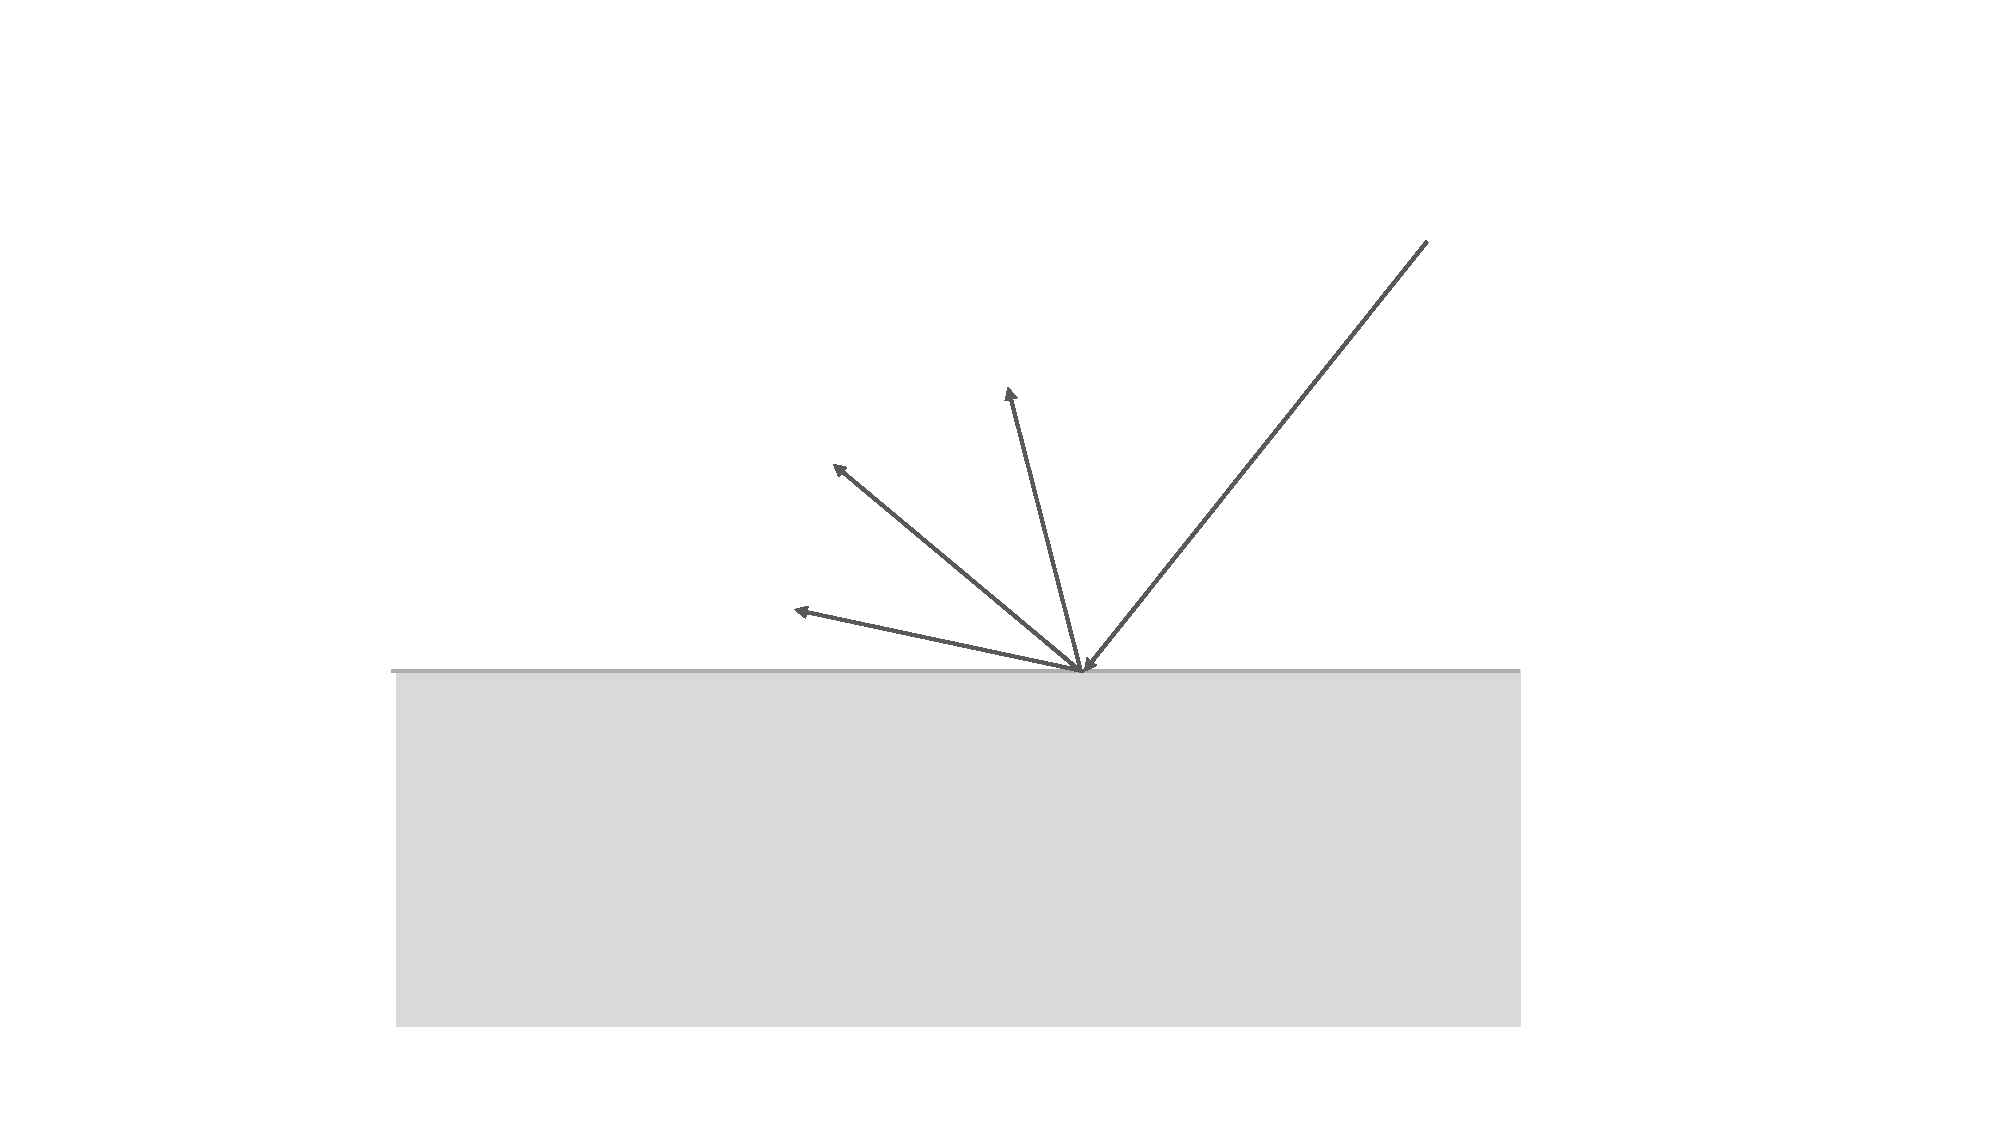
\includegraphics[width=0.46\linewidth]{figs/BRDF.pdf}
  }
  \hspace{0.04\linewidth}
  \subfloat[BSSRDF]{
    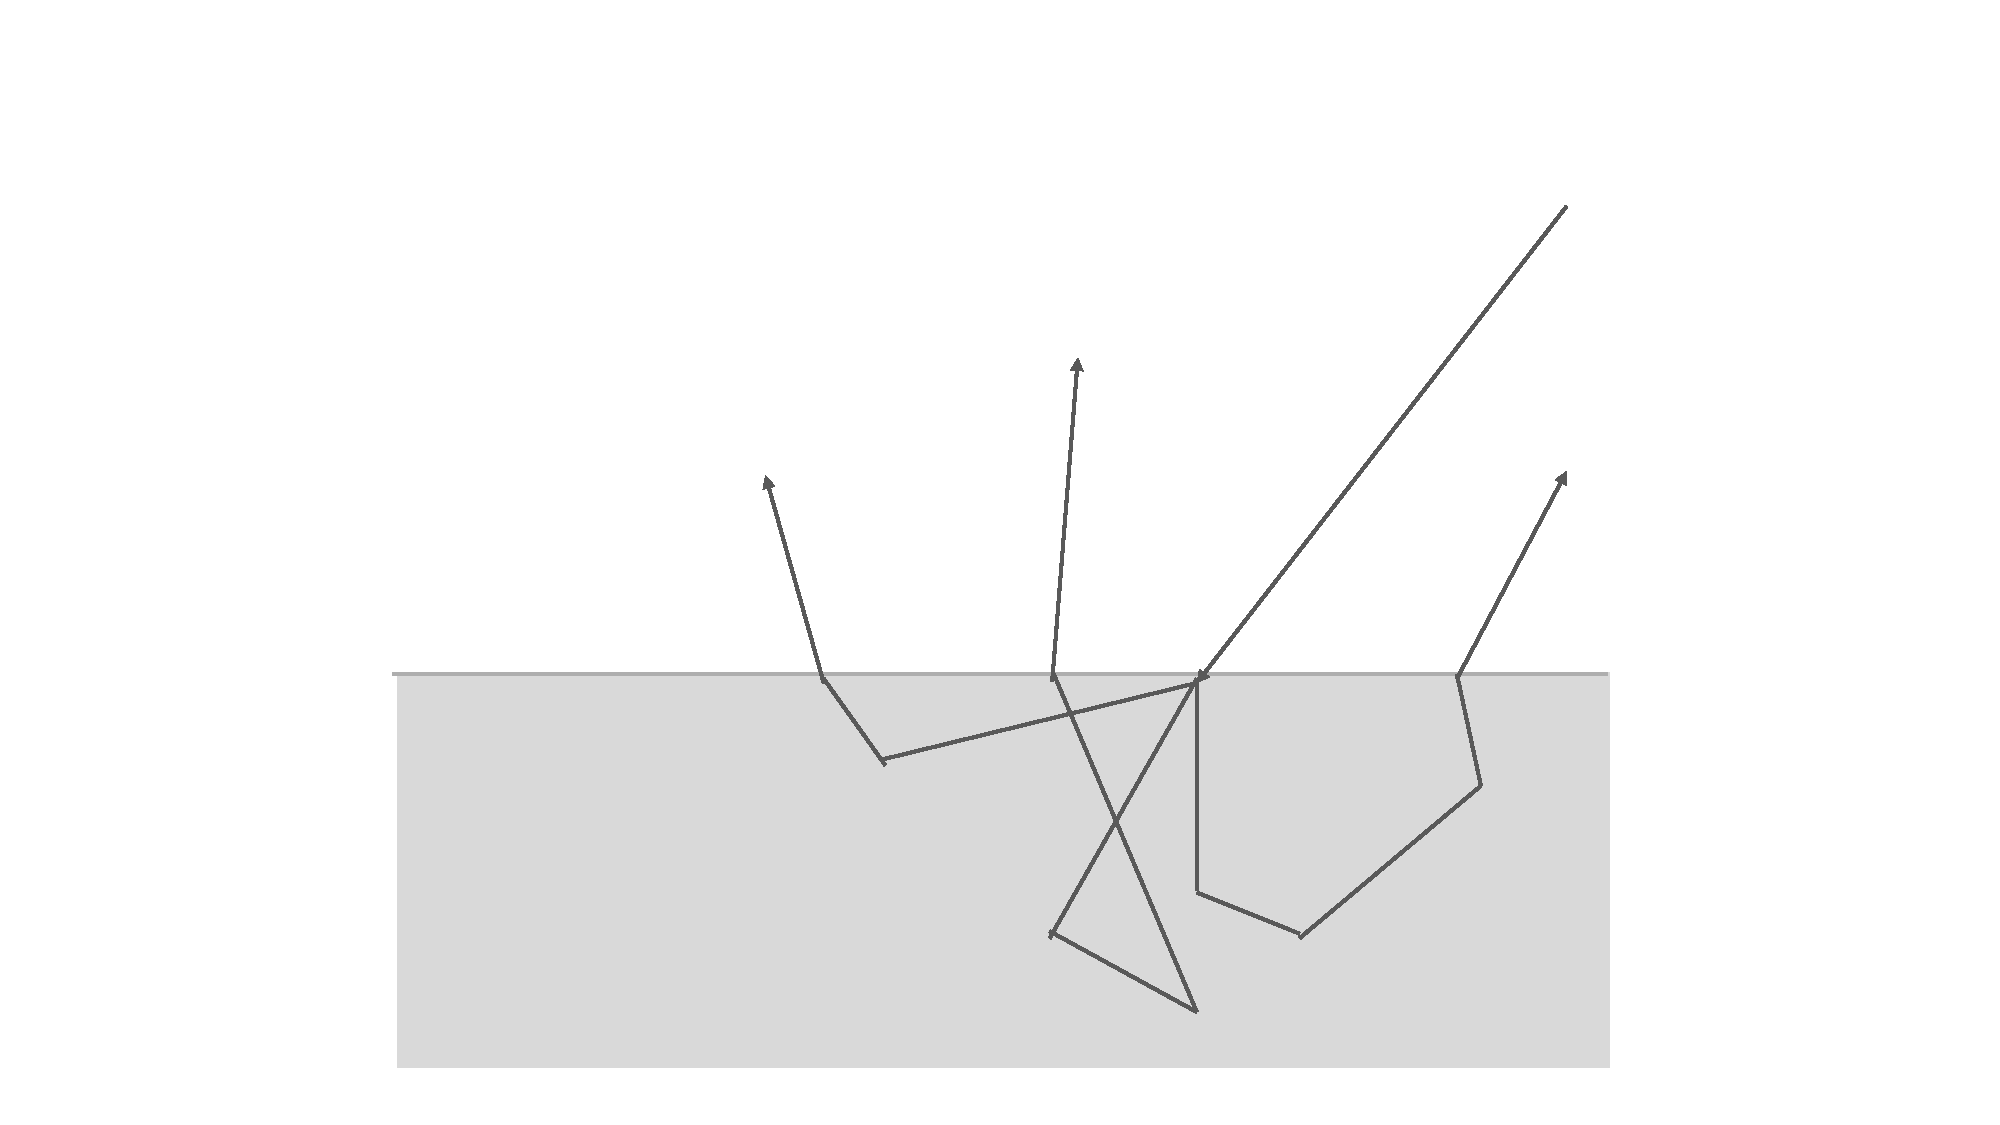
\includegraphics[width=0.46\linewidth]{figs/BSSRDF.pdf}
  }
  \caption{BRDF と BSSRDF による光輸送モデルの違いの概念図（文献\cite{Jensen2001Dipole}を参考に作成）。}
  \label{fig:brdf_bssrdf}
\end{figure}
\section{皮膚の表面下散乱モデル}
皮膚は，表皮，真皮，皮下組織といった
複数の層から構成される多層構造を持ち，
各層で異なる吸収・散乱特性を示す。
これらを厳密に扱うためには，
放射輸送方程式を解く必要があるが，
計算コストが高いため，
実用的なレンダリングでは近似モデルが用いられる。

皮膚表面下散乱モデルの代表的な研究として，
Donner と Jensen による研究
\cite{Donner2006Spectral}
が挙げられる。
この研究では，
皮膚内部での光の散乱を
スペクトル領域で扱うBSSRDFモデルが提案されており，
皮膚に特有な色変化や透明感を
高い精度で再現できることが示されている。
同手法は拡散近似に基づいており，
計算効率と写実性の両立を実現した点で，
皮膚表現に関する多くの後続研究の基盤となっている。

\begin{figure}[tb]
  \centering
  
\includegraphics[width=0.8\linewidth]{figs/chot_1.jpg}
  \caption{人間の皮膚における多層構造と光輸送の概念図。
皮膚は表皮，真皮，皮下組織など
複数の層から構成されており，
各層で光の吸収および散乱特性が異なる。
このような層構造を考慮することで，
皮膚表面下散乱のより現実的な表現が可能となる。}
  \label{fig:skin_layers}
\end{figure}
さらに，
Weyrich らによる研究
\cite{Weyrich2008Layered}
では，
皮膚を多層構造かつ空間的に不均質な媒質として扱う
反射モデルが提案されている。
この研究では，
実測データに基づいて皮膚の層構造を取得し，
層ごとに異なる光学特性を持たせることで，
より現実的な皮膚表現を実現している。

これらの研究は，
皮膚が一様な媒質ではなく，
層構造や空間的な不均質性を持つことを示しており，
皮膚表面下散乱モデルの高度化に大きく貢献している。

\section{毛髪・髭表現に関する研究}
毛髪表現に関する研究は，
主に頭髪を対象として発展してきた。
毛髪一本一本を幾何的に表現し，
異方的な反射モデルを適用することで，
写実的な見えを再現する手法が数多く提案されている。

一方で，
顔に存在する髭は，
頭髪と比較して短く，
高密度に分布するという特徴を持つ。
そのため，
毛髪一本単位での厳密な表現は，
計算コストの観点から
実用的でない場合が多い。

多くの皮膚表面下散乱モデルでは，
皮膚内部の光学特性に焦点が当てられており，
皮膚表面付近に局所的に分布する構造物，
例えば髭のような毛髪要素については，
明示的には扱われていない。
その結果，
髭が存在する領域においても
皮膚のみの場合と同様の散乱特性が適用され，
見えの違いが十分に表現されないという問題がある。

\section{本研究の位置づけ}
以上のように，
皮膚表面下散乱に関する研究は数多く存在する一方で，
髭のような局所的な構造物が
皮膚表面下散乱に与える影響を，
簡潔かつ実用的に取り込む手法は
十分に検討されていない。

本研究は，
Donner と Jensen による
皮膚表面下散乱モデルや，
Weyrich らによる
多層・不均質皮膚モデルを基盤としつつ，
髭という局所的不均質性を
髭密度という形で表現し，
皮膚表面下散乱モデルに組み込む点に特徴がある。

毛髪一本単位の厳密なモデル化を行うのではなく，
髭の分布を密度マップとして集約することで，
計算効率を保ちながら，
髭の存在による見えの変化を
連続的に表現することを目指す。

次章では，
本研究で提案する
髭密度を考慮した皮膚表面下散乱モデルについて
詳しく説明する。













\chapter{提案手法}
\label{cha:method}

本章では，本研究で提案する「髭密度を考慮した皮膚表面下散乱モデル」について詳述する。
本研究の目的は，人間の顔表面において局所的に分布する髭の影響を考慮し，
皮膚表面下散乱の見えをより現実的に再現することである。

本章では，まず本研究で扱う問題設定を整理し，
次にベースとなる皮膚表面下散乱モデルについて説明する。
その後，髭密度を導入した混合反射モデルと，
それを実現するための髭密度マップ生成手法を示す。
最後に，提案モデルをモンテカルロパストレーシングに統合する
レンダリングアルゴリズムについて説明する。

\subsection{問題設定}
本研究では，人間の顔表面における光輸送を対象とし，
特に髭が存在する領域において生じる表面下散乱の見えの変化に着目する。

従来の皮膚表面下散乱モデルでは，
皮膚を一様な多層媒質として近似する場合が多く，
局所的な構造物である髭の分布による影響は
明示的には考慮されてこなかった。
しかし実際の人間の顔では，
髭の密度は空間的に大きく変化しており，
これにより光の吸収量や散乱距離が領域ごとに異なる。
\begin{figure}[tb]
  \centering
  \subfloat[髭なし]{
    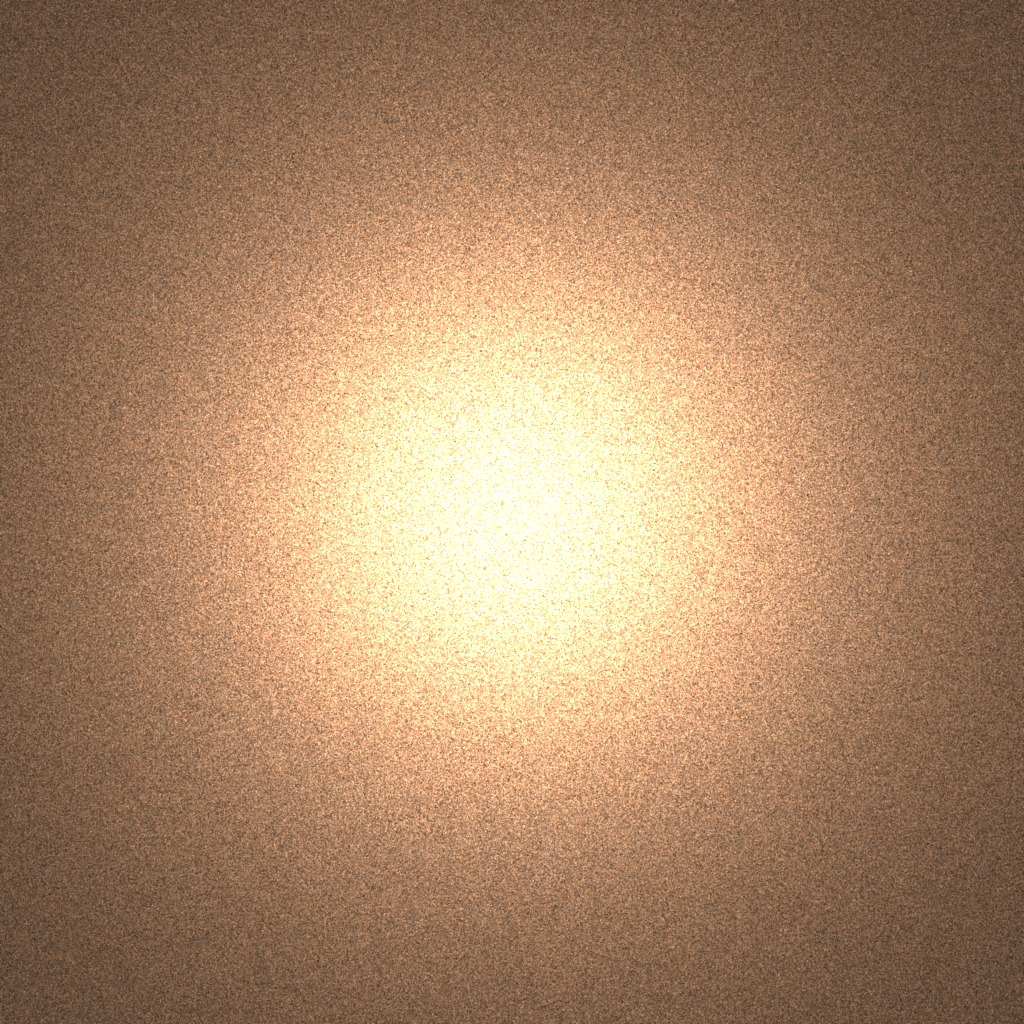
\includegraphics[width=0.46\linewidth]{figs/out_no_beard.png}
  }
  \hspace{0.04\linewidth}
  \subfloat[髭あり]{
    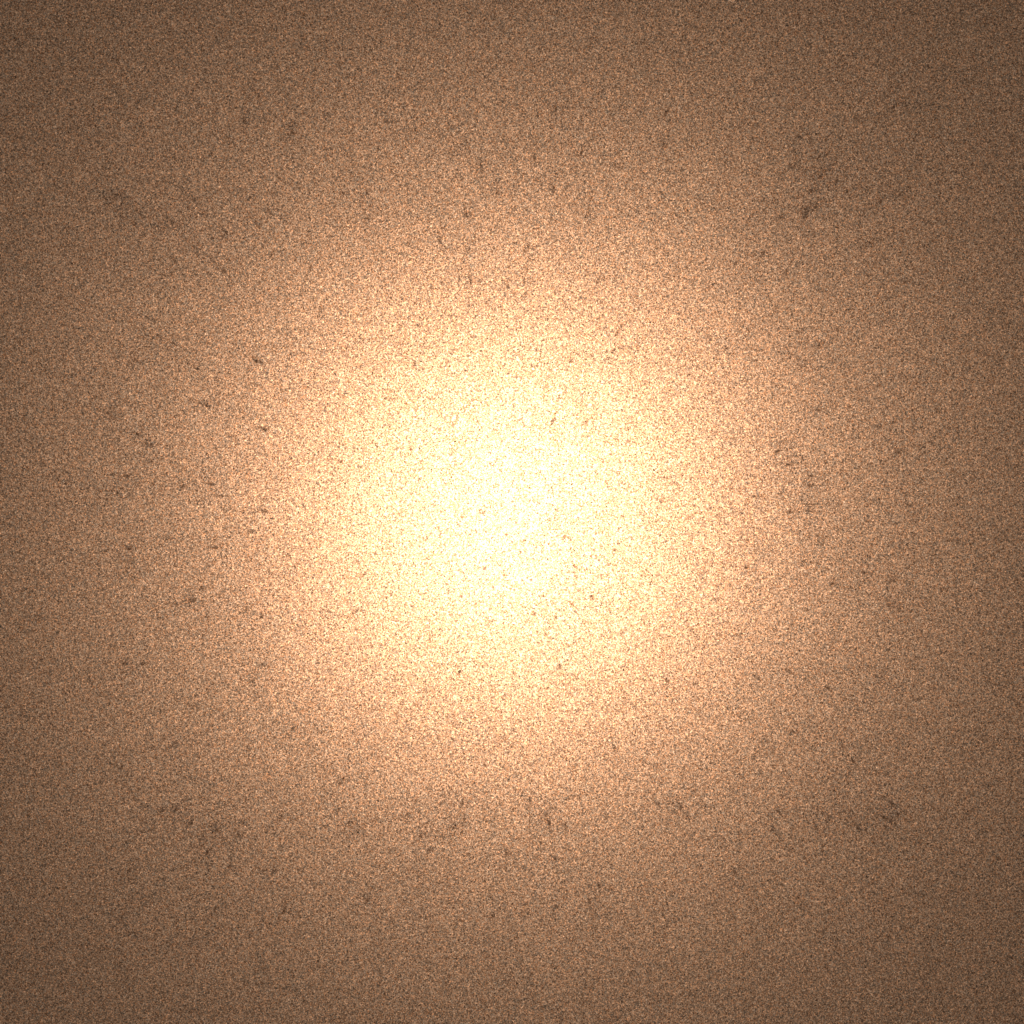
\includegraphics[width=0.46\linewidth]{figs/out_beard.png}
  }
  \caption{Mitsuba による髭なし／髭ありシーンのレンダリング結果。
髭が存在する領域では，皮膚のみの場合と比較して，
光のにじみや明度分布が変化する。}
  \label{fig:beard_effect}
\end{figure}

このような不均質性を無視したモデルでは，
髭の生えている領域において
光のにじみが過度に強く現れたり，
逆に暗部が不自然に減衰するなどの問題が生じる。
そこで本研究では，
皮膚表面下散乱モデルに髭密度という空間的に変化するパラメータを導入し，
髭の存在による影響を連続的に表現することを目的とする。

\subsection{皮膚表面下散乱モデル}
皮膚内部における光の散乱は，
光が表面から入射し，内部で複数回散乱した後，
異なる位置から出射する現象として観測される。
このような光輸送を記述するため，
本研究では双方向表面下散乱反射率分布関数
(Bidirectional Surface Scattering Reflectance Distribution Function: BSSRDF)
を用いる。

BSSRDF は，入射位置 $\mathbf{x}_i$，
入射方向 $\omega_i$，
出射位置 $\mathbf{x}_o$，
出射方向 $\omega_o$ に依存する関数として定義され，
次式で表される。

\begin{equation}
S(\mathbf{x}_i, \omega_i, \mathbf{x}_o, \omega_o)
=
\frac{dL_o(\mathbf{x}_o, \omega_o)}
     {d\Phi_i(\mathbf{x}_i, \omega_i)}
\end{equation}


本研究では，
既存研究において広く利用されている
拡散近似に基づく皮膚BSSRDFモデルをベースモデルとして採用する。
拡散近似は，
散乱回数が十分に多い場合に成立する近似であり，
人間の皮膚のような強散乱媒質に対して
計算効率と再現性の両立が可能である。
\begin{figure}[tb]
  \centering
  
\includegraphics[width=0.8\linewidth]{figs/chot.pdf}
    \caption{皮膚表面下散乱における光輸送の概念図。
    光は入射点 $\mathbf{x}_i$ から皮膚内部に侵入し，
    複数回散乱した後，異なる位置 $\mathbf{x}_o$ から出射する。}


  \label{fig:sss_transport}
\end{figure}

\subsection{髭密度を考慮した混合モデル}
髭が存在する皮膚表面では，
皮膚のみの場合と比較して，
光の吸収および散乱特性が変化する。
髭は主にメラニンを多く含む毛髪繊維で構成されており，
皮膚表面付近において光を吸収・遮蔽する役割を果たす。

本研究では，
この影響を明示的にモデル化するため，
皮膚モデルと髭モデルを
髭密度に基づいて混合する手法を提案する。
各表面点において髭密度を
$d \in [0,1]$ と定義し，
$d=0$ は髭の存在しない皮膚，
$d=1$ は髭の影響が最大である状態を表す。

出射点における表面下散乱特性は，
次式に示すように，
皮膚モデルと髭モデルの線形結合として表現される。

\begin{equation}
S_{\mathrm{mix}}
=
(1 - d)\, S_{\mathrm{skin}} + d\, S_{\mathrm{beard}}
\end{equation}

線形混合を採用した理由は，
髭密度が連続的に変化する領域において，
反射特性が不連続に変化することを防ぎ，
安定したレンダリング結果を得るためである。
また，本手法は既存のBSSRDFモデルを拡張する形で実装可能であり，
計算コストの増加を最小限に抑えられるという利点を持つ。
\subsubsection{髭密度を出射点で評価する理由}
本研究では，髭密度 $d$ を入射点ではなく，
表面下散乱後の出射点において評価する。
これは，本研究で用いるBSSRDFが，
光の入射位置と出射位置が異なる現象を記述するモデルであり，
最終的な見えに直接影響を与えるのが出射点であるためである。

皮膚表面下散乱では，
光は皮膚内部を伝播した後，
周囲の別の位置から出射する。
そのため，入射点近傍における髭の有無よりも，
実際に光が出射する位置周辺の構造が，
最終的な放射輝度に強く影響する。

仮に入射点の髭密度のみを用いた場合，
皮膚内部で大きく移動した光に対しても，
入射点の情報が適用されることになり，
髭分布と見えの対応関係が不自然になる可能性がある。
特に，髭の境界付近では，
入射点と出射点で密度が大きく異なる場合があり，
これがアーティファクトの原因となる。

以上の理由から，本研究では，
表面下散乱サンプリングによって決定された出射点において
髭密度を参照し，
混合反射モデルを適用する設計とした。
\subsubsection{髭モデルの反射特性}
本研究における髭モデル $S_{\mathrm{beard}}$ は，
髭一本一本の幾何構造を直接表現するものではなく，
髭の存在によって生じる
皮膚表面下散乱特性の変化を近似的に表現するモデルである。

髭は皮膚表面付近に分布する毛髪繊維であり，
光に対して主に吸収および遮蔽の役割を果たす。
その結果，髭が存在する領域では，
皮膚内部を長距離伝播する光の寄与が減少し，
有効的な散乱距離が短くなる傾向がある。

本研究では，
この効果を簡潔に表現するため，
髭モデルを
皮膚モデルと比較して
吸収の強い，
かつ拡散半径の小さい反射モデルとして定義する。
これにより，
髭密度が高い領域では，
表面下散乱による光のにじみが抑制され，
より引き締まった見えが得られる。

このように，
$S_{\mathrm{beard}}$ は
毛髪一本単位の物理モデルではなく，
皮膚表面下散乱に対する
髭の影響を集約的に表現する
有効モデルとして位置づけられる。

\subsubsection{線形混合モデルにおける近似と限界}
本研究で採用した混合モデルは，
髭密度 $d$ に基づいて皮膚モデルと髭モデルを線形に補間するものである。
この定式化は実装が容易であり，
既存の表面下散乱モデルとの親和性が高い一方で，
いくつかの近似を含んでいる。

まず，本研究では，
髭一本一本の物理的形状，
すなわち太さ，長さ，曲率，および生え方の方向分布といった
高次の幾何学的要因を明示的には考慮していない。
実際の髭は円柱状の繊維構造を持ち，
その太さや長さは光の遮蔽率や散乱特性に影響を与える。
しかし，これらの要因を直接モデル化するためには，
毛髪一本単位でのジオメトリ表現や，
異方的な散乱モデルを導入する必要があり，
計算コストが著しく増大する。

また，髭同士の重なりによる自己遮蔽や，
毛髪間で生じる多重散乱効果も本研究では考慮していない。
これらの効果は，
高密度な髭領域において特に重要となるが，
正確に扱うためには，
毛髪集合体を体積媒質として扱うような
高度なモデルが必要となる。

本研究では，
これらの高次効果をすべて
髭密度という単一のスカラー量に集約することで，
皮膚表面下散乱に対する髭の影響を
低次元かつ連続的に表現することを選択した。
この近似により，
レンダリングの安定性を保ちつつ，
髭分布に応じた見えの変化を
実用的な計算時間で再現することが可能となる。

以上より，本研究の線形混合モデルは，
物理的に厳密な毛髪モデルではなく，
皮膚表面下散乱への影響を簡潔に取り込むための
近似モデルとして位置づけられる。
\subsubsection{他の混合モデルとの比較}
髭密度に基づく反射モデルの構築にあたり，
線形混合以外の手法についても検討を行った。
例えば，
非線形関数による補間や，
指数関数を用いた減衰モデル，
あるいは有効散乱係数を
髭密度に応じて直接変化させる手法が考えられる。

しかし，非線形混合モデルでは，
髭密度のわずかな変化に対して
反射特性が急激に変化する場合があり，
密度分布が滑らかな領域においても
不安定なレンダリング結果を生じることが確認された。
また，有効散乱係数を直接操作する手法では，
物理パラメータの解釈が困難となり，
既存の皮膚表面下散乱モデルとの比較が難しくなる。

これに対して，
線形混合モデルは，
髭密度と反射特性の関係が直感的であり，
密度が連続的に変化する場合でも
安定した結果を得ることができる。
以上の理由から，
本研究では線形混合モデルを採用した。


\subsection{髭密度マップの生成}
髭密度は，
顔表面上の各位置に対して定義されるスカラー量であり，
テクスチャマップとして表現される。
本研究では，
髭ジオメトリの分布情報から
密度マップを自動生成する。

\begin{figure}[tb]
  \centering
  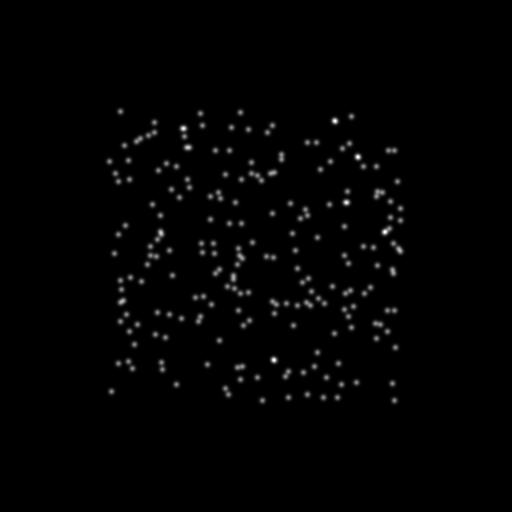
\includegraphics[width=0.8\linewidth]{figs/beard_density_xz.jpg}
\caption{髭ジオメトリから生成された髭密度マップの例。
密度マップはUV空間上に定義され，
レンダリング時に各表面位置の密度値を取得するために用いられる。}



  \label{fig:beard_density_map}
\end{figure}
まず，髭ジオメトリを入力として，
各皮膚表面点に対する近傍領域を定義する。
次に，その領域内に含まれる髭の本数や占有率を評価し，
正規化された密度値として $d$ を算出する。
生成された密度値はUV空間に投影され，
テクスチャマップとして保存される。

この密度マップは，
レンダリング時において
表面位置に対応する密度値を高速に取得するために用いられる。
\subsubsection{密度マップの解像度と平滑化処理}
髭密度マップの解像度は，
見えの再現性と計算効率の両立において
重要な要素である。
解像度が低すぎる場合，
髭分布の境界が粗くなり，
表面下散乱結果に
ブロック状のアーティファクトが生じる。
一方で，過度に高解像度な密度マップは，
メモリ使用量の増加や
キャッシュ効率の低下を招く。

本研究では，
これらのトレードオフを考慮し，
実験的に十分な精度が得られる解像度を採用した。
また，密度マップ生成時には，
局所的なばらつきを抑制するため，
平滑化処理を施している。
この処理により，
髭の疎密が連続的に変化する領域においても，
自然な見えを維持することが可能となる。

なお，密度マップは
髭ジオメトリに基づく近似であるため，
完全に正確な物理量ではない。
しかし，本研究では，
この近似が視覚的な品質に与える影響は限定的であり，
提案手法の有効性を評価する上で
十分であると判断した。

\subsection{レンダリングアルゴリズム}
提案手法を用いたレンダリングは，
モンテカルロ法に基づくパストレーシングによって行う。
出射放射輝度は次式により数値的に推定される。

\begin{equation}
L_o(\mathbf{x}_o, \omega_o)
\approx
\frac{1}{N}
\sum_{k=1}^{N}
\frac{f_k\, L_i(\omega_k)\, \cos\theta_k}
     {p(\omega_k)}
\end{equation}

本研究では，
この推定を表面下散乱サンプリングに組み込み，
サンプリングされた出射点において
髭密度を参照することで，
混合BSSRDFを適用する。

提案手法を用いたレンダリングの処理手順を以下に示す。

\begin{enumerate}
  \item レイと皮膚表面との交差判定
  \item 交差点における髭密度の取得
  \item 髭密度に基づく混合反射モデルの決定
  \item 表面下散乱に基づく出射点サンプリング
  \item 放射輝度の計算
\end{enumerate}

以上の処理を
モンテカルロパストレーシングに統合することで，
髭密度に応じた表面下散乱表現を実現する。
\subsection{計算コストと実装上の考察}
提案手法では，
髭密度マップの参照と
混合反射モデルの計算が追加されるが，
これらはいずれも定数時間で実行可能である。
そのため，
レンダリング全体の計算量は，
従来のBSSRDFを用いたパストレーシングと
同程度に保たれる。

特に，
髭をジオメトリとして直接扱わず，
密度マップとして集約した点は，
計算量削減の観点から重要である。
毛髪一本単位の交差判定や散乱計算を行う場合と比較して，
提案手法は
実用的な計算時間でのレンダリングを可能にする。

\chapter{評価実験}

\section{検証の目的}
本研究では，
第3章で提案した
髭密度を考慮した皮膚表面下散乱モデルの妥当性を検証することを目的とする。
提案手法は，
髭一本一本の幾何構造を直接扱うのではなく，
髭の分布を髭密度というスカラー量として近似し，
この密度に基づいて皮膚モデルと髭モデルを混合する点に特徴がある。

皮膚表面下散乱に対する髭の影響は，
髭自身が形成する遮蔽や影，
毛の太さや深さ，
配置のばらつきなど，
多くの要因が複雑に関与する現象である。
そのため，
髭を幾何構造として忠実に扱う場合，
計算コストが高くなるだけでなく，
得られる結果が
必ずしも安定した挙動を示すとは限らない。

本研究では，
このような複雑な要因をすべて厳密にモデル化するのではなく，
髭の分布を密度という抽象化された量として扱うことで，
表面下散乱特性を
安定かつ連続的に制御することを目指している。
したがって，
提案モデルの妥当性を評価する上で重要なのは，
幾何的な髭モデルを正確に再現できているかどうかではなく，
この抽象化が
設計意図どおりの振る舞いを
実際に生み出しているかを確認することである。

特に本章では，
髭密度の変化に応じて，
表面下散乱の空間的広がりや
放射束分布が，
不自然な不連続や破綻を生じることなく，
滑らかかつ安定して変化するかどうかを
モデルの妥当性の指標とする。

本章で検証する問いは，以下の2点である。
\begin{enumerate}
  \item 髭密度に基づく線形混合モデルが，
        表面下散乱分布を不自然に破綻させることなく，
        密度変化に対して連続的かつ安定に応答するか。
  \item 髭を幾何構造として直接扱った場合に観測される挙動と比較して，
        髭密度モデルが，
        表面下散乱特性を制御・評価するための
        実用的かつ妥当な抽象化として機能しているか。
\end{enumerate}

これらの問いに答えるため，
本章では定量的および定性的な評価を行う。
定量的評価では，
点光源入射時における
表面下散乱の空間分布を計測し，
入射点からの距離に対する減衰特性を比較する。
また，
定性的評価では，
髭密度を変化させたレンダリング画像を比較し，
見えの変化や
不自然なアーティファクトの有無を確認する。

\begin{enumerate}
  \item 髭密度を用いた線形混合が，
        表面下散乱分布を不自然に破綻させることなく，
        密度変化に対して連続に応答するか。
  \item 髭を幾何構造として直接扱う場合と比較して，
        髭密度による近似が，
        表面下散乱特性を評価する上で妥当な抽象化となっているか。
\end{enumerate}

これらの問いに答えるため，
本章では定量的および定性的な評価を行う。
定量的評価では，
点光源入射時における
表面下散乱の空間分布を計測し，
入射点からの距離に対する減衰特性を比較する。
また，
定性的評価では，
髭密度を変化させたレンダリング画像を比較し，
見えの変化やアーティファクトの有無を確認する。





\section{実験環境および共通設定}
本章における評価実験では，
提案した髭密度を考慮した皮膚表面下散乱モデルの挙動を
定量的に観測するため，
単純化した検証シーンを用いる。
レンダリングにはモンテカルロ法に基づくパストレーシングを用い，
表面下散乱の計算には
第3章で述べたBSSRDFモデルを組み込んだ。

定量評価では，
幾何形状や陰影の影響を排除し，
表面下散乱の空間的広がりのみを評価するため，
無限平面上に皮膚モデルを配置し，
点光源を垂直方向から入射させる構成を用いた。
この構成により，
入射点を基準とした距離依存の散乱特性を
明確に観測することが可能となる。

照明条件，反射モデルのパラメータ，
およびサンプル数は，
すべての実験条件において共通とし，
比較対象間で条件が一致するように設定した。
これにより，
観測される差異は
髭の有無やモデル化手法の違いに起因するものとして
解釈することができる。
実験シーンの概要を
図\ref{fig:exp_setup}に示す。
\begin{figure}[tb]
  \centering
  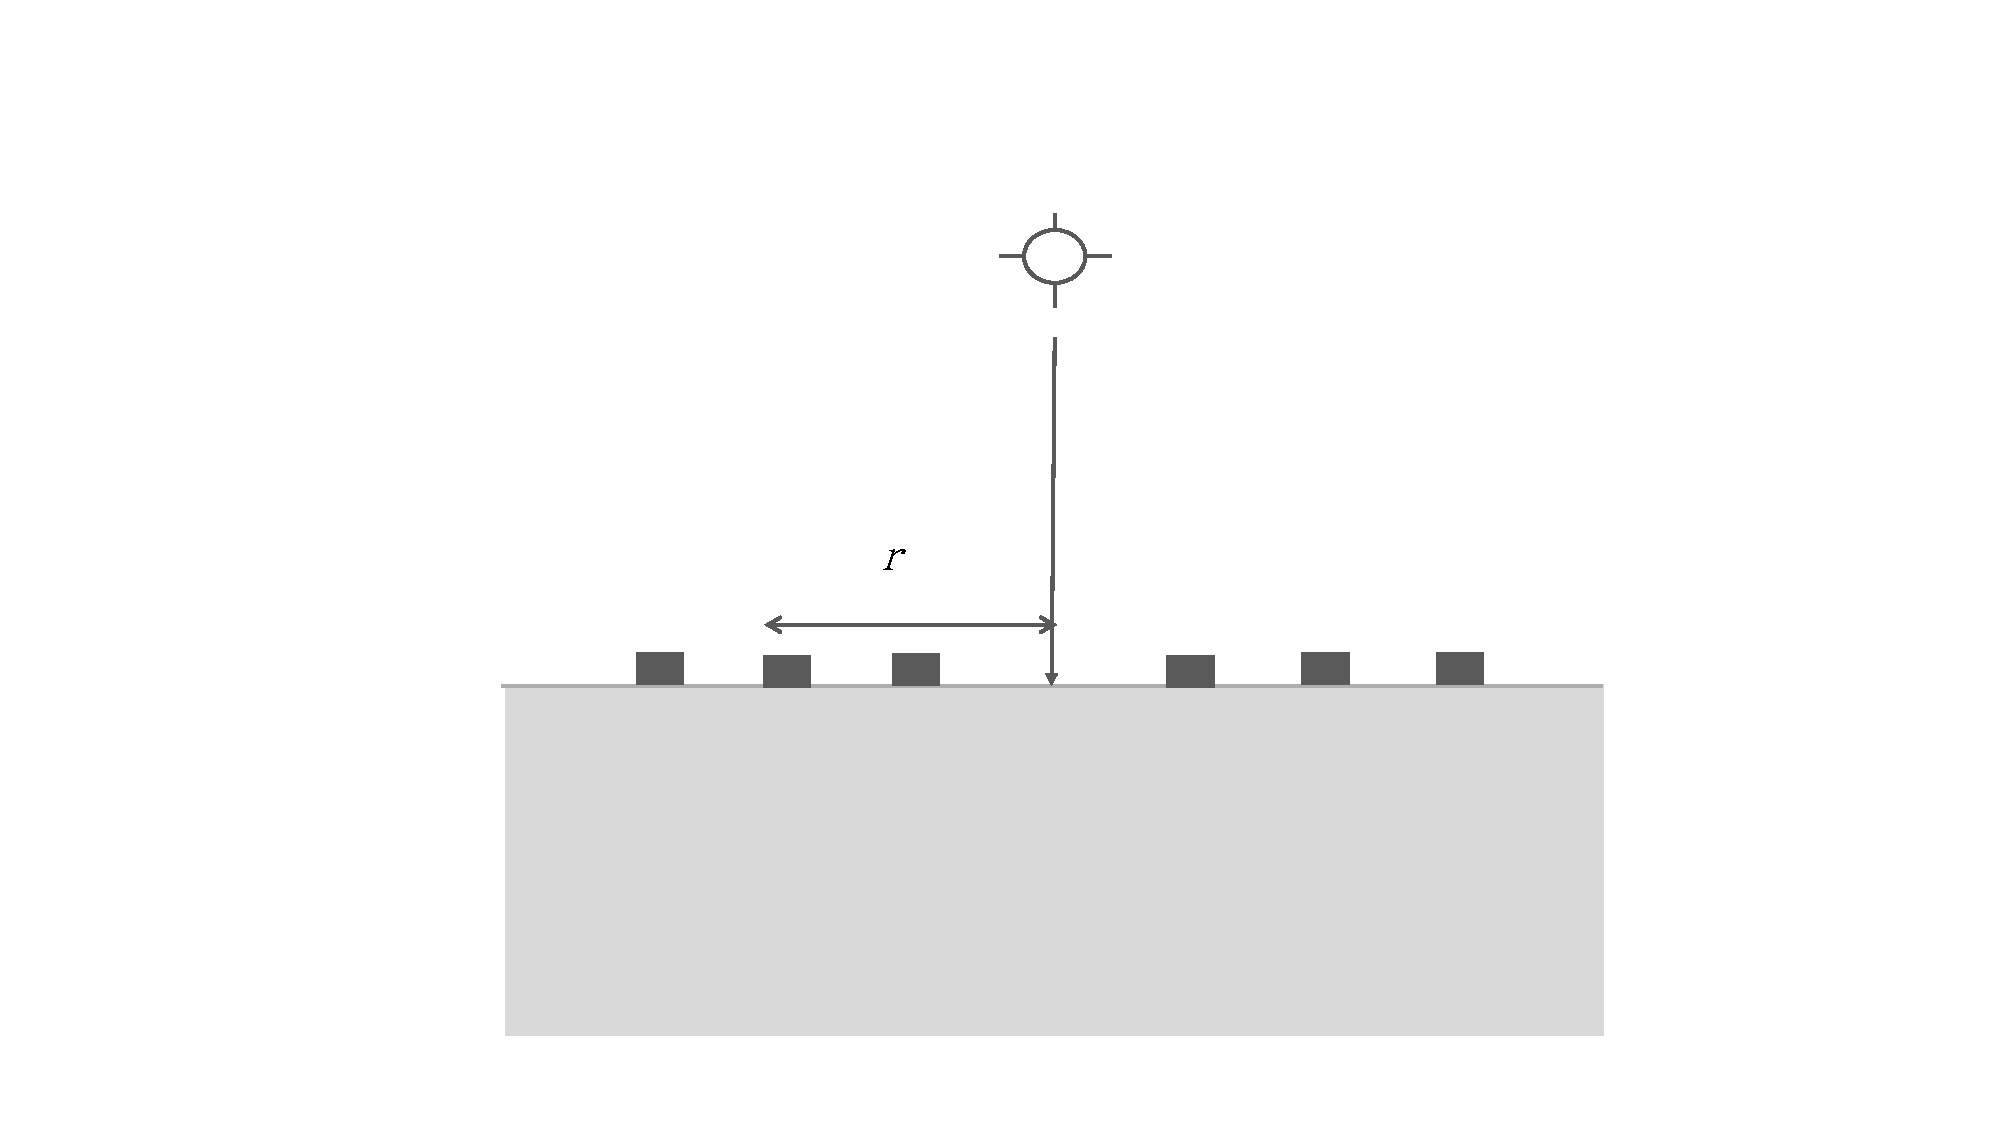
\includegraphics[width=0.8\linewidth]{figs/scene_setup.pdf}
  \caption{評価シーンの構成。無限平面上の入射点に点光源を垂直入射させ，
  入射点を中心とした半径 $r$ のリング上に配置した観測点で $R_d(r)$ を計測する。}
  \label{fig:exp_setup}
\end{figure}


\section{表面下散乱分布 $R_d(r)$ の計測}
\label{sec:rd_measure}
本節では，
表面下散乱の空間的な広がりを評価するために用いた
指標および計測方法について述べる。

\subsection{評価指標の定義}
\label{sec:rd_definition}
表面下散乱の広がりを評価する指標として，
入射点から距離 $r$ だけ離れた位置における
放射束分布 $R_d(r)$ を用いる。
$R_d(r)$ は，
点光源が皮膚表面に垂直入射した際に，
入射点を中心とする距離 $r$ の位置から
出射する放射束の分布を表す量であり，
表面下散乱による光の拡散特性を反映する。

本実験では，
表面上の同心円リングに沿って
複数の評価点を配置し，
各点における入射放射束を照度計によって計測した。
各距離 $r$ における $R_d(r)$ は，
円周方向にサンプリングした値の平均として算出する。
これにより，
角度方向のばらつきを抑え，
距離依存性に着目した評価が可能となる。

また，
分布形状の比較を容易にするため，
得られた $R_d(r)$ は
全距離にわたる面積積分が 1 となるよう正規化している。
この正規化により，
絶対的なエネルギー量ではなく，
距離方向の減衰特性そのものに着目した比較を行うことができる。

\subsection{計測シーンおよび手順}
\label{sec:rd_procedure}
計測は，
無限平面上に配置した皮膚モデルに対して，
点光源を垂直方向から入射させる構成で行った。
入射点を原点とし，
距離 $r$ に応じて
同心円状に評価点を配置することで，
幾何形状による影響を排除し，
表面下散乱の広がりのみを観測できるようにした。

各距離 $r$ において，
円周方向に複数点をサンプリングし，
それらの平均値を $R_d(r)$ として記録した。
評価点の配置および
計測手順の概念図は割愛する。


\section{幾何的髭モデルによる基礎検証}
\label{sec:geom_beard}
本節では，
提案する髭密度モデルの評価に先立ち，
髭を幾何構造として直接表現した場合の
表面下散乱分布の挙動を確認するための
基礎的な検証について述べる。

本検証では，
髭を円柱状の幾何構造としてモデル化し，
皮膚平面の内部に埋め込んだ。
円柱は皮膚表面に対して垂直に配置され，
その位置および本数は固定とした。
このような構成により，
髭を一本一本の幾何として忠実に扱った場合に，
表面下散乱分布 $R_d(r)$ がどのように変化するかを観測する。

計測方法および評価指標は，
前節で述べたものと同一とし，
髭なしの皮膚モデルと，
幾何的髭モデルを含む場合とで
$R_d(r)$ を比較した。
これにより，
モデル化手法以外の要因を排除した
直接的な比較が可能となる。

幾何的髭モデルを用いた場合の
$R_d(r)$ の計測結果を
髭なしの場合とともに
図\ref{fig:geom_beard_rd}に示す。
\begin{figure}[tb]
  \centering
  
\includegraphics[width=0.8\linewidth]{figs/chot_2.jpg}
  \caption{幾何的髭モデルと髭なしの場合の $R_d(r)$ 比較結果。}
  \label{fig:geom_beard_rd}
\end{figure}
本節では，
これらの結果を
観測事実として提示するに留め，
得られた分布の意味や
提案モデルとの関係についての考察は
次章で行う。
\section{評価設計の成立確認}
\label{sec:eval_ready}

本節では，
前節までに構築した評価指標および計測手法が，
自作レンダラー環境においても
適切に機能することを確認する。

自作レンダラーを用い，
無限平面上の皮膚モデルに対して
点光源を入射させる構成において，
入射点からの距離 $r$ に応じた
表面下散乱分布 $R_d(r)$ を計測した。
その結果，
髭なし，髭モデル，および両者を混合した条件のいずれにおいても，
$R_d(r)$ が非ゼロかつ連続な値として得られ，
数値的に安定した分布を取得できることを確認した。

また，
条件間で分布形状の比較を行うため，
得られた $R_d(r)$ に対して
\[
\int 2\pi r R_d(r)\,dr = 1
\]
となるよう面積積分による正規化を施した。
この正規化により，
絶対的なエネルギー量の違いを排除し，
距離方向の減衰特性に着目した比較が可能となる。

以上より，
本研究で用いる評価指標および計測手法は，
自作レンダラー環境においても
一貫して適用可能であり，
次章における結果の提示および考察に
用いることができる形式のデータが得られた。


\chapter{結果}
\label{cha:results}

\section{表面下散乱分布の計測結果}
\label{sec:results_rd}

本節では，
前章で確立した評価手法を用いて得られた
自作レンダラーによる計測結果を示す。
\begin{figure}[H]
  \centering
  
\includegraphics[width=0.8\linewidth]{figs/chot.pdf}
  \caption{髭なし，髭モデル，混合モデルにおける正規化表面下散乱分布 $R_d(r)$ の比較。}
  \label{fig:rd_norm_compare}
\end{figure}

図\ref{fig:rd_norm_compare}は，
髭なしの皮膚モデル，
髭モデル，
および両者を混合したモデルに対して計測した
正規化後の表面下散乱分布 $R_d(r)$ を比較したものである。
いずれの分布も面積積分が 1 となるよう正規化されており，
分布形状の違いに着目した比較が可能である。

図より，
各条件において $R_d(r)$ の分布形状に差が見られ，
特に混合モデルの分布は，
髭なしモデルと髭モデルの中間的な挙動を示している。
また，
いずれの分布も距離 $r$ に対して滑らかに変化しており，
計測結果がノイズや発散に支配されていないことが確認できる。

これらの結果は，
髭の有無やモデルの違いが
表面下散乱分布に反映されていることを示している。
次節では，
これらの分布の違いについて考察を行う。
\section{考察}

\section{幾何的な髭モデルによる検証の限界}

本研究では当初，
髭を円柱などの幾何形状として明示的に配置したシーンを用い，
表面下散乱の放射輝度分布を計測することで，
髭が皮膚表面下散乱に与える影響を直接的に評価することを試みた。

しかし，
このような幾何的髭モデルによる検証では，
いくつかの課題が明らかとなった。

まず，
髭の配置位置や深さ，太さのわずかな違いによって，
計測される放射輝度分布が大きく変動する傾向が確認された。
これは，
髭が作る自己遮蔽や影，
さらに皮膚内部での多重散乱との相互作用が複雑に絡み合うためであり，
幾何的に厳密なモデルであっても，
安定した再現性を得ることが困難であることを示している。

また，
髭一本一本を幾何形状として扱う場合，
シーン内のプリミティブ数が急激に増加し，
計算コストが大きくなるという実用上の問題も無視できない。
このため，
幾何モデルは理論的には詳細な表現が可能である一方，
実際のレンダリングや検証においては，
不安定かつ高コストな手法となる。

以上より，
幾何的な髭モデルは，
「髭が表面下散乱に影響を与えうる」ことを確認する手段としては有効であるが，
その影響を安定的かつ制御可能な形で評価する基準モデルとして用いることは，
必ずしも適切ではないと考えられる。

\section{髭密度モデルによる表面下散乱制御の妥当性}

これに対し，
本研究で提案した髭密度モデルは，
髭の幾何構造そのものを直接扱うのではなく，
髭の分布を表面上のスカラー量として近似し，
皮膚モデルと髭モデルを線形に混合するという設計を採用している。

第\ref{sec:results_rd}節で示した結果より，
この髭密度に基づく混合モデルでは，

\begin{itemize}
  \item 放射輝度分布 $R_d(r)$ が不自然に破綻することなく，
  \item 髭密度の増加に応じて，
        表面下散乱の広がりが連続的に変化する
\end{itemize}

ことが確認された。

特に注目すべき点は，
放射輝度分布を正規化した後においても，
髭密度の違いによる分布形状の差が明確に現れている点である。
これは，
単に全体のエネルギー量が変化しているのではなく，
光の空間的な拡散特性そのものが変化していることを示している。

この結果は，
髭密度という単純化された指標を用いた線形混合であっても，
表面下散乱の挙動を十分に特徴づけられることを示唆しており，
提案モデルの設計判断が妥当であることを支持している。

\section{幾何モデルと密度モデルの関係性について}

本研究において重要なのは，
髭密度モデルが幾何的髭モデルを厳密に再現することではない。
むしろ，
髭が表面下散乱に与える影響は，

\begin{itemize}
  \item 髭の太さ
  \item 配置密度
  \item 皮膚内部への侵入深さ
  \item 髭自身が作る影や遮蔽
\end{itemize}

といった多くの要因が複雑に関係しており，
これらをすべて厳密にモデル化することは現実的ではない。

このような背景を踏まえると，
髭密度モデルは，
幾何的に複雑な要因を一つのスカラー量に集約し，
その影響を現象論的に捉えるための抽象化であると位置付けられる。

第\ref{sec:results_rd}節で示した差分実験の結果から，
幾何的髭モデルと髭密度モデルの間には，
放射輝度分布の変化傾向において共通点が見られた。
このことは，
密度モデルが幾何モデルの詳細を再現していないにもかかわらず，
髭の存在による影響を方向性として適切に捉えていることを示している。

したがって，
提案モデルは，
「物理的に完全な髭モデル」ではなく，
「表面下散乱に対する髭の影響を安定かつ制御可能な形で表現するための実用的モデル」
として位置付けることができる。

\section{本研究の位置付けと限界}

本研究で提案した髭密度モデルは，
計算コストと表現力のバランスを重視した近似モデルであり，
すべての髭表現を正確に再現できるものではない。
特に，
個々の髭が作る鋭い影や，
髭同士の相互遮蔽といった効果については，
本モデルでは明示的に扱っていない。

一方で，
顔全体のレンダリングやインタラクティブな応用を想定した場合，
髭の影響を密度という形で扱い，
表面下散乱の広がりを連続的に制御できる点は，
実用上大きな利点である。

以上より，
本研究のモデルは，
高精度な物理再現を目的とするモデルとは異なる立場にあり，
実用的な皮膚レンダリングにおける
新たな設計指針を提示するものであると考えられる。

\section{まとめ}

本章では，
幾何的な髭モデルと比較しながら，
髭密度に基づく表面下散乱モデルの妥当性について考察を行った。

その結果，

\begin{itemize}
  \item 髭は表面下散乱の放射輝度分布に影響を与えること
  \item 幾何モデルによる厳密な評価は不安定かつ高コストであること
  \item 髭密度モデルは，
        その影響を安定的かつ連続的に制御可能であること
\end{itemize}

が確認された。

これらの知見は，
髭のような微細構造を持つ要素を含む皮膚表現において，
密度に基づく近似モデルが有効な選択肢となり得ることを示している。



\chapter{まとめと今後の課題}

\section{まとめ}

本研究では，
髭の存在が皮膚表面下散乱に与える影響を，
実用的な計算コストで表現することを目的として，
髭密度を用いた表面下散乱モデルを提案した。

従来のアプローチでは，
髭を一本一本の幾何構造として扱う必要があり，
その結果，
計算コストの増大や，
配置条件に強く依存した不安定な挙動が問題となる。
これに対し，
本研究では，
髭の分布を表面上のスカラー量である「髭密度」として近似し，
皮膚モデルと髭モデルを線形に混合することで，
表面下散乱特性を制御する手法を採用した。

評価実験では，
点光源入射時における放射輝度分布 $R_d(r)$ を用いて，
髭なしの場合，
幾何的な髭モデルを含む場合，
および提案した髭密度モデルの場合を比較した。
その結果，
髭の存在が表面下散乱の空間的な広がりに影響を与えることが確認され，
特に髭密度モデルにおいては，
分布形状が不自然に破綻することなく，
髭密度の変化に応じて連続的に制御できることが示された。

また，
幾何的な髭モデルとの比較から，
提案モデルは髭の詳細な幾何構造を厳密に再現するものではないものの，
髭の存在による表面下散乱特性の変化を，
方向性として適切に捉えていることが確認された。
このことから，
髭密度という抽象化は，
表面下散乱に対する髭の影響を安定かつ実用的に扱うための
有効な近似であると結論付けられる。

以上より，
本研究は，
髭のような微細構造を持つ要素を含む皮膚レンダリングにおいて，
密度に基づく近似モデルが有効であることを示し，
実用的な表面下散乱表現に対する一つの設計指針を提示した。

\section{今後の課題}

本研究で提案した髭密度モデルは，
計算コストと表現力のバランスを重視した近似モデルであり，
いくつかの課題が残されている。

まず，
本モデルでは，
髭の影響をスカラーの密度値として表現しているため，
髭の方向性や太さのばらつき，
髭同士の相互遮蔽といった効果は明示的に扱っていない。
これらの要素を考慮することで，
より多様な髭表現に対応できる可能性がある。

次に，
幾何的な髭モデルとの対応関係については，
本研究では主に定性的および差分的な比較に留まっている。
将来的には，
髭の太さや埋め込み深さを系統的に変化させた幾何モデルとの比較を行い，
幾何的要因と髭密度との関係をより定量的に分析することが課題として挙げられる。

また，
本研究では静的な髭密度マップを用いたが，
実際の顔表現では，
部位ごとの密度差や，
成長・剃毛・スタイリングによる時間的変化が存在する。
提案モデルは，
密度マップを差し替えることでこれらの変化に対応可能であるため，
動的な髭密度を扱う拡張も今後の課題である。

さらに，
本手法は髭を対象として検討を行ったが，
同様の考え方は，
産毛や皮膚表面の微細な繊維構造など，
他の微細要素を含む表現にも応用できる可能性がある。
これらへの適用可能性を検討することも，
今後の展開として考えられる。

以上の課題に取り組むことで，
髭密度に基づく表面下散乱モデルの表現力と汎用性をさらに高めることが期待される。

\chapter*{謝辞}
\addcontentsline{toc}{chapter}{謝辞}
本稿の執筆に際し，終始あたたかく丁寧な相談，ご指導をいただいた青山学院大学理工学部情報テクノロジー学科○○○○教授に深く感謝申し上げます．
また，研究の方針や問題解決にあたって様々な助言・ご指導をしていただいた○○研究室の茅野氏，宇城氏，峯氏に深く感謝申し上げます．そして，実験に協力していただいた被験者の皆様に御礼申し上げます．

\begin{flushright}
2024年1月29日
\\
手久野　呂次
\end{flushright}


\newpage
\nocite{*}
\bibliographystyle{unsrt}
\bibliography{ref}




%\chapter*{質疑応答}

\note{卒研発表後に，発表当日の質疑で提起された質問とそれに対する答えをまとめてください．}

\begin{table}[h]
\centering
\large
\begin{tabular}{ll}

& 伊藤　雄一　情報テクノロジー学科　教授 \\ \hline
\multicolumn{1}{|l|}{Q} & \multicolumn{1}{l|}{\begin{tabular}[c]{@{}l@{}}\parbox{37zw}{\strut{}
今後より高度なGPTが発表された場合でも，提案法は有効と考えられるか？あるいは何か改善すべき点があるか？
\strut}\end{tabular}} \\ \hline
\multicolumn{1}{|l|}{A} & \multicolumn{1}{l|}{\begin{tabular}[c]{@{}l@{}}\parbox{37zw}{\strut{}
提案法では，XXXという考え方を利用しているため，どんなにGPTが高度になっても対応できると考えられる．
\strut}\end{tabular}} \\ \hline

\end{tabular}
\end{table}

\begin{table}[h]
\centering
\large
\begin{tabular}{ll}

& Martin J. D\"{u}rst 情報テクノロジー学科　教授 \\ \hline
\multicolumn{1}{|l|}{Q} & \multicolumn{1}{l|}{\begin{tabular}[c]{@{}l@{}}\parbox{37zw}{\strut{}
「ChatGPT と人を見分ける」ということがタイトルにあるが，評価実験では ChatGPT によって生成された文章だけを入力対象にしている．人が書いた文章を入力にしてそれが人によって書かれたものであると判定できることを確認しなくて良いか？極端な話，毎回ランダムに 95\% の確率で ChatGPT と答えれば，評価実験と同じ結果を得ることができるのではないか？
\strut}\end{tabular}} \\ \hline
\multicolumn{1}{|l|}{A} & \multicolumn{1}{l|}{\begin{tabular}[c]{@{}l@{}}\parbox{37zw}{\strut{}
人が書いた文章を入力とした場合，高確率で人だと答えることができるが，締め切り直前にその実験結果を卒業研究論文に含めることができなかった．修正した現在のバージョンではその実験も追加した．
\strut}\end{tabular}} \\ \hline

\end{tabular}
\end{table}

\begin{table}[h]
\centering
\large
\begin{tabular}{ll}

& 大原　剛三　情報テクノロジー学科　教授 \\ \hline
\multicolumn{1}{|l|}{Q} & \multicolumn{1}{l|}{\begin{tabular}[c]{@{}l@{}}\parbox{37zw}{\strut{}
評価に使っている文章はほとんどが時事ニュースに関するものに見えるが，他の種類の文章は対象にしなくて良いのか？判定できている理由として，ChatGPT では学習が必要なために，最新の時事ニュースとの間にタイムラグがあるからだ，ということは考えられないか？
\strut}\end{tabular}} \\ \hline
\multicolumn{1}{|l|}{A} & \multicolumn{1}{l|}{\begin{tabular}[c]{@{}l@{}}\parbox{37zw}{\strut{}
タイムラグを利用しているわけではないと思うが，確かに他のクラスの文章での評価が必要．今後の課題とする．
\strut}\end{tabular}} \\ \hline

\end{tabular}
\end{table}

\begin{table}[h]
\centering
\large
\begin{tabular}{ll}

& 伊藤　弘大　情報テクノロジー学科　助教 \\ \hline
\multicolumn{1}{|l|}{Q} & \multicolumn{1}{l|}{\begin{tabular}[c]{@{}l@{}}\parbox{37zw}{\strut{}
Omission を実行する際にパラメータ $O$ があるが，いくつに設定しているか？
\strut}\end{tabular}} \\ \hline
\multicolumn{1}{|l|}{A} & \multicolumn{1}{l|}{\begin{tabular}[c]{@{}l@{}}\parbox{37zw}{\strut{}
3.14に設定されている．
\strut}\end{tabular}} \\ \hline

\end{tabular}
\end{table}



\end{document}
